\documentclass{beamer}
\usepackage{beamerthemesplit}
\usepackage{wrapfig}
\usetheme{SPbGU}
\usepackage{pdfpages}
\usepackage{amsmath}
\usepackage{cmap} 
\usepackage[T2A]{fontenc} 
\usepackage[utf8]{inputenc}
\usepackage[english,russian]{babel}
\usepackage{indentfirst}
\usepackage{amsmath}
\usepackage{tikz}
\usepackage{multirow}
\usepackage[noend]{algpseudocode}
\usepackage{algorithm}
\usepackage{algorithmicx}
\usepackage[export]{adjustbox}
\usepackage{graphicx}
\usetikzlibrary{shapes,arrows}
\usepackage{fancyvrb}
\newtheorem{rutheorem}{Теорема}
\newtheorem{ruproof}{Доказательство}
\newtheorem{rudefinition}{Определение}
\newtheorem{rulemma}{Лемма}
\beamertemplatenavigationsymbolsempty

\title[]{Библиотека YC.QuickGraph: поиск путей с КС-ограничениями в графах}
%\subtitle[]{Опциональный подзаголовок}
% То, что в квадратных скобках, отображается в левом нижнем углу. 
\institute[СПбГУ]{
Санкт-Петербургский государственный университет \\
Кафедра системного программирования }

% То, что в квадратных скобках, отображается в левом нижнем углу.
\author[Свитков Сергей]{Свитков Сергей Андреевич, 344 группа \\
  % У научного руководителя должна быть указана научная степень
  \and  
    {\bfseries Научный руководитель:} ст. пр., к. ф-м н. Григорьев С.В. \\ }
  % Для курсовой не обязателен. Должна быть указана должность или ученая степень

\date{27 апреля 2017г.}

\definecolor{orange}{RGB}{179,36,31}

\begin{document}
{
% Лого университета или организации, отображается в шапке титульного листа
\begin{frame}
  \begin{center}
  {
\includegraphics[width=1.5cm]{pictures/SPbGU_Logo.png}}
  \end{center}
  \titlepage
\end{frame}
}

\begin{frame}[fragile]
  \transwipe[direction=90]
  \frametitle{Введение}
  \begin{itemize}
    \item Ориентированные графы с метками на рёбрах
    \begin{itemize}
        \item Графовые базы данных
        \item Социальные графы
        \item Биоинформатика
        \item ...
    \end{itemize}
    \item Пути в подобных графах могут представлять интерес
    \begin{itemize}
        \item Последовательность из меток на рёбрах
    \end{itemize}
    \item КС-грамматики
    \begin{itemize}
        \item Позволяют задать КС-язык
        \item КС-язык можно использовать как язык запросов
    \end{itemize}
    \item Поиск интересующих строчек в графе
    \begin{itemize}
        \item Последовательность меток на ребрах в графе выводима в заданном языке
    \end{itemize}
  \end{itemize}
\end{frame}
            
\begin{frame}
  \transwipe[direction=90]
  \frametitle{Обзор существующих решений}
  \begin{itemize}
    \item Большинство существующих языков запросов к графам --- регулярные
    \begin{itemize}
        \item Cypher (Neo4J)
        \item Gremlin (Titan)
    \end{itemize}
    \item Контекстно-свободные языки запросов
    \begin{itemize}
        \item Большое количество теории
        \item Существуют реализации, но с очень ограниченной функциональностью
    \end{itemize}
  \end{itemize}
\end{frame}

\begin{frame}
  \transwipe[direction=90]
  \frametitle{Conjunctive Context-Free Path Queries}
  \begin{itemize}
    \item 2014, Jelle Hellings
    \item Обобщение существующего регулярного языка CRPQ до КС-языка CCFPQ
    \item Позвляет использовать КС-языки для запросов
    \item Использует CYK для синтаксического анализа графов
    \item Результат --- КС-отношение \(R = (N,\, n,\, m)\), где \(N\) --- нетерминал, из которого выводим путь из вершины \(n\) в \(m\)
  \end{itemize}
  
  \begin{itemize}
    \item Минусы
    \begin{itemize}
      \item Нет практической реализации
      \item Представление результата только в одном формате
    \end{itemize}
  \end{itemize}
\end{frame}

\begin{frame}
  \transwipe[direction=90]
  \frametitle{Subgraph Queries by Context-free Grammars}
  \begin{itemize}
    \item 2008, Petteri Sevon and Lauri Eronen
    \item Применение КС-запросов в биоинформатике
    \item Для синтаксического анализа используется Earley Parser 
    \item Результат --- связный подграф, порожденный множеством путей, строки из меток на ребрах которых выводимы из заданной грамматики
  \end{itemize}
  
  \begin{itemize}
    \item Минусы
    \begin{itemize}
      \item Алгоритм имеет приемлемое время работы только на небольших входных данных
      \item Проблемы при наличии циклов в графе
      \item Предложенный алгоритм представляет результат только в одном формате
    \end{itemize}
  \end{itemize}
\end{frame}

\begin{frame}
  \transwipe[direction=90]
  \frametitle{Ослабленный синтаксический анализ динамически формируемых выражений на основе алгоритма GLL}
  \begin{itemize}
    \item 2016, Рагозина А.К.
    \item Синтаксический анализ регулярной аппроксимации (конечный автомат, граф), основанный на GLL
    \item Обрабатывает большие входные данные 
    \item Работает с графами, рёбра которых помечены токенами --- численными значениями
    \item Результат --- лес разбора всех путей в графе, выводимых в заданном языке (SPPF)
    \item Реализован в рамках YaccConstructor (.NET)
  \end{itemize}
\end{frame}

\begin{frame}
  \transwipe[direction=90]
  \frametitle{Обзор существующих решений}
  \begin{itemize}
    \item Существующие библиотеки для работы с графами для .NET
    \begin{itemize}
        \item QuickGraph --- заброшен в 2011
        \item YC.QuickGraph --- основывается на QuickGraph, поддерживается сейчас
    \end{itemize}
  \end{itemize}
\end{frame}

\begin{frame}
  \transwipe[direction=90]
  \frametitle{Итоги обзора}
  \begin{itemize}
    \item Существенные минусы у существующих практических реализаций (один формат результата, слишком наивные алгоритмы, ...)
    \item Хочется представить реализацию, не имеющую перечисленных недостатков
    \item Представление результата запроса должно быть возможно в нескольких форматах:
    \begin{itemize}
        \item Кратчайший путь
        \item Подграф
        \item Множество путей
        \item КС-отношение
    \end{itemize}
    \item Можно использовать результаты работы Рагозиной А. К. для синтаксического анализа графов, если преобразовать пользовательские объекты на рёбрах графа в токены
  \end{itemize}
\end{frame}

% Обязательный слайд: четкая формулировка цели данной работы и постановка задачи
% Описание выносимых на защиту результатов, процесса или особенностей их достижения и т.д.
\begin{frame}
  \transwipe[direction=90]
  \frametitle{Постановка задачи}
  \textbf{Целью} работы является создание библиотеки, позволяющей выполнять КС-запросы к графам и предоставлять пользователю результат запроса в различных форматах\\ 
  \textbf{Задачи}:
  \begin{itemize}
    \item Разработать архитектуру решения
    \item Реализовать библиотеку
    \item Провести тестирование библиотеки
    \item Представить конечный результат в виде NuGet-пакета для использования в языках платформы .NET
  \end{itemize}
\end{frame}

\begin{frame}
  \transwipe[direction=90]
  \frametitle{Результаты}
  На данный момент достигнуты следующие результаты
  \begin{itemize}
    \item Изучена предметная область
    \item Спроектирована архитектура решения
    \item Реализовано
    \begin{itemize}
        \item Поддержка задания грамматики строкой
        \item Возможность задания графа с пользовательскими объектами на рёбрах
        \item Поддержка преобразования пользовательского объекта к токену
        \item Начальный прототип: позволяет задать запрос, граф и получить результат --- SPPF
    \end{itemize}
  \end{itemize}
\end{frame}

\begin{frame}
  \transwipe[direction=90]
  \frametitle{Архитектура решения}
  Упрощенная архитектура решения:
  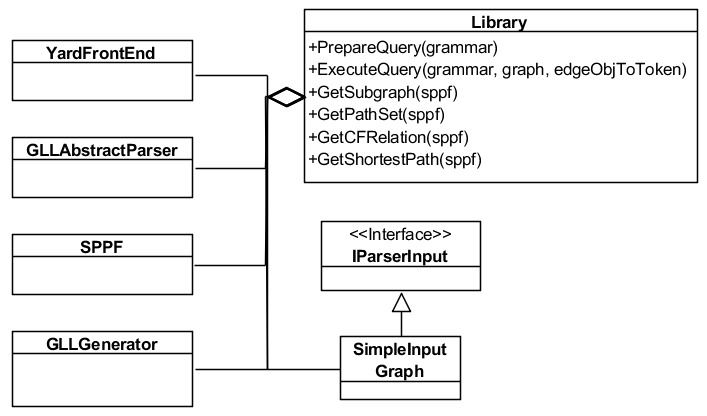
\includegraphics[max size={\textwidth}{\textheight}]{pictures/arch.png}
\end{frame}

\begin{frame}
  \transwipe[direction=90]
  \frametitle{Прототип решения}
  Процесс исполнения запроса:
  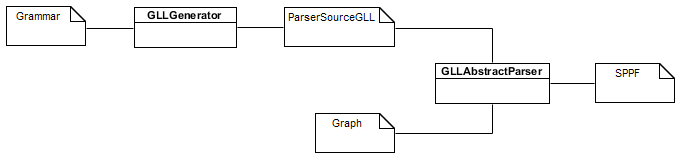
\includegraphics[max size={\textwidth}{\textheight}]{pictures/pipe.png}
\end{frame}

\begin{frame}
  \transwipe[direction=90]
  \frametitle{Дальнейшие планы}
  \begin{itemize}
    \item Реализовать преобразования SPPF к различным форматам
    \item Протестировать полученное решение
    \item Написать документацию, собрать NuGet-пакет
  \end{itemize}
\end{frame}

\end{document}